\section{Evaluation}
\label{sec:evaluation}

\subsection{Visual Odometry to record Racing Lines}
Visual Odometry has many theoretical advantages over GPS. The amount of data points received is a lot higher, as it produces 1 position per frame, which could realistically result in 30 - 60 positional updates per second, wheres GPS usually produces 1 point per second. This high amount of points makes a detailed comparison and analysis a lot easier, as curves appear mostly smooth instead of having only a couple of straight lines, as seen in figure \ref{fig:vo_gps_comp}.

\begin{figure}[!ht]
	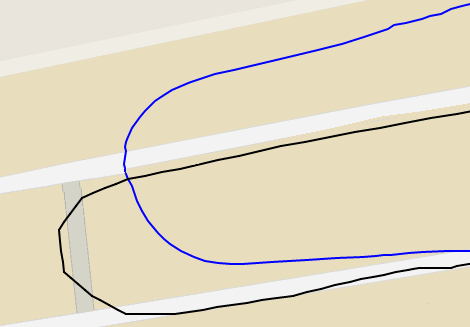
\includegraphics[width=\textwidth]{VO_corner_comp}
	\caption{Visual Odometry (blue) produces much smoother curves than GPS (black), but can be erroneous}
	\label{fig:vo_gps_comp}
\end{figure}

Consequently, VO is capable of detecting very small movements. A racing car driving at 100 km/h travels ~28 meters forward every second. The lateral movement, i.e. driving from one side of the track to the other or through corners, is much slower. So, assuming a driver takes 2 seconds to cross a 10 m wide track, we would get one positional update every 17 cm at 30 frames per second. 

Obviously, this is 30 times better than GPS because of the higher speed alone, but also the GPS standard (NMEA 0183) is only accurate to $\frac{1}{60 000}$ of a degree. The distance between two degrees of latitude is 110 km, the distance between two meridians at 51° (position of Berlin) 70 km. That means the accuracy in North-South direction is 1.8 m and in East-West direction 1.2 m. If the Region of Interest (ROI) of our camera image has a real-world width of 30 m and the recording has Full-HD resolution, the accuracy of VO would be 3 cm.
Another advantage of Visual Odometry is that it doesn't rely on external sources, like satellites, and is in general mostly independent of the area it is used. After all, even the Mars Rovers used this algorithm to navigate. Especially in forests, rural areas and tunnels, GPS is either inaccurate or not usable at all. The camera-based approach still works when GPS fails.
So all in all, VO is able of extracting a very detailed depiction of the racing line, even in remote areas. However, the algorithms used are fairly expensive.
A mobile-range computer (like the Nvidia Jetson TX1) can achieve an average frame rate of about 8 frames per second at a resolution of 672 x 376 px. This is in theory still better than GPS, but it is an average value, potentially becoming a lot slower in feature-dense areas, like forests, and especially corners. The reason VO slows down in corners is, that rather than tracking already existent features points it has to search new points much more frequently than on straights, because the scenery changes much quicker.
Additionally, VO can only determine a relative difference to the last calculated position. This means, that potential errors, like too shallow corner angles, will result in faulty results throughout the entire path. This can also be seen in figure \ref{fig:vo_gps_comp}. The incoming and outgoing straights should be close to parallel, but the VO image detected them at an angle. If this turn would be repeated, the error would cause the line to not be consistently at the same position every time, without further processing.

\subsection{Usefulness of Racing Line Comparison}
\begin{itemize}
  \item professional drivers can achieve similar lap times with very different racing lines
  \item however amateur and intermediate drivers can learn a lot from more skilled drivers
\end{itemize}


\clearpage
